%allgemeine Formatangaben
\documentclass[
 a4paper, 										% Papierformat
 12pt,												% Schriftgröße
 ngerman, 										% für Umlaute, Silbentrennung etc.
 titlepage,										% es wird eine Titelseite verwendet
 oneside, 										% einseitiges Dokument
 captions=nooneline,					% einzeilige Gleitobjekttitel ohne Sonderbehandlung wie mehrzeilige Gleitobjekttitel behandeln
 numbers=noenddot,						% Überschriften-??Nummerierung ohne Punkt am Ende
 parskip=half,									% zwischen Absätzen wird eine halbe Zeile eingefügt
 ]{scrartcl}


% Anpassung an Landessprache
\usepackage[ngerman]{babel}	

\usepackage[T1]{fontenc}	
\usepackage[utf8]{inputenc}	
\usepackage{textcomp} 																% Euro-Zeichen und andere
\usepackage[babel,german=quotes]{csquotes}						% Anführungszeichen
\RequirePackage[ngerman=ngerman-x-latest]{hyphsubst} 	% erweiterte Silbentrennung

\usepackage{tocloft} %Wird benötigt damit das veränderte Counterverhalten nicht mit Text überlappt!
\usepackage{etoolbox} %Url Umbruch im Bibtex!

% Befehle aus AMSTeX für mathematische Symbole z.B. \boldsymbol \mathbb
\usepackage{amsmath,amsfonts}

% Zeilenabstände und Seitenränder 
\usepackage{setspace}
\usepackage{geometry}

% Einbinden von JPG-Grafiken
\usepackage{graphicx}

% zum Umfließen von Bildern
% Verwendung unter http://de.wikibooks.org/wiki/LaTeX-Kompendium:_Baukastensystem#textumflossene_Bilder
\usepackage{floatflt}

% Verwendung von vordefinierten Farbnamen zur Colorierung
% Palette und Verwendung unter http://kitt.cl.uzh.ch/kitt/CLinZ.CH/src/Kurse/archiv/LaTeX-Kurs-Farben.pdf
\usepackage[usenames,dvipsnames]{color} 

% Tabellen
\usepackage{array}
\usepackage{longtable}

% einfache Grafiken im Code
% Einführung unter http://www.math.uni-rostock.de/~dittmer/bsp/pstricks-bsp.pdf
%\usepackage{pstricks}


% Quellcodeansichten
%\usepackage{verbatim}
%\usepackage{moreverb} 											% für erweiterte Optionen der verbatim Umgebung
% Befehle und Beispiele unter http://www.ctex.org/documents/packages/verbatim/moreverb.pdf
%\usepackage{listings} 											% für angepasste Quellcodeansichten siehe
% Kurzeinführung unter http://blog.robert-kummer.de/2006/04/latex-quellcode-listing.html



% verlinktes und Farblich angepasstes Inhaltsverzeichnis
\usepackage[pdftex,
colorlinks=true,
linkcolor=InterneLinkfarbe,
urlcolor=ExterneLinkfarbe]{hyperref}
\usepackage[all]{hypcap}

% URL verlinken, lange URLs umbrechen
\usepackage{url}

% sorgt dafür, dass Leerzeichen hinter parameterlosen Makros nicht als Makroendezeichen interpretiert werden
\usepackage{xspace}

% Beschriftungen für Abbildungen und Tabellen
%\usepackage{caption}

%\usepackage{chngcntr}
%Ändert counterverhalten von figure, table usw..

% Entwicklerwarnmeldungen entfernen
%\usepackage{scrhack}
% Glossar und Abbildungsverzeichnis
%\usepackage[
%nonumberlist, %keine Seitenzahlen anzeigen
%acronym,      %ein Abkürzungsverzeichnis erstellen
%toc          %Einträge im Inhaltsverzeichnis
%]      %im Inhaltsverzeichnis auf section-Ebene erscheinen
%{glossaries}
\usepackage{makeidx}
\makeindex

\usepackage{amsmath, amssymb}

\usepackage[printonlyused]{acronym}					% einbinden der verwendeten Latex-Pakete
\newcommand{\qq}[1]{\glqq{#1\grqq{}}} %Gänsefüßchen
\newcommand{\idx}[1]{#1\index{#1} } % Index drucken und schreiben

\onehalfspacing 							% 1,5facher Zeilenabstand

\definecolor{InterneLinkfarbe}{rgb}{0.1,0.1,0.3} 	% Farbliche Absetzung von externen Links
\definecolor{ExterneLinkfarbe}{rgb}{0.1,0.1,0.7}	% Farbliche Absetzung von internen Links

% Einstellungen für Fußnoten:
\captionsetup{font=footnotesize,labelfont=sc,singlelinecheck=true,margin={5mm,5mm}}

% Quellenangaben Stil
\bibliographystyle{alphadin}

%Ausschluss von Schusterjungen
\clubpenalty = 10000
%Ausschluss von Hurenkindern
\widowpenalty = 10000


% Beispiel für eine Listings-Codeumbebungen
% Bei mehreren Definitionen empfielt sich das auslagern in eine externe Datei
\lstloadlanguages{C++}
\lstset{
	frame=tb,
	framesep=5pt,
	basicstyle=\footnotesize\ttfamily,
	showstringspaces=false,
	keywordstyle=\ttfamily\bfseries %\color{CadetBlue},
	identifierstyle=\ttfamily,
	stringstyle=\ttfamily %\color{OliveGreen},
	%commentstyle=\color{GrayBlue},
%	rulecolor=\color{Gray},
	xleftmargin=5pt,
	xrightmargin=5pt,
	aboveskip=\bigskipamount,
	belowskip=\bigskipamount
} 

%Den Punkt am Ende jeder Beschreibung deaktivieren
\renewcommand*{\glspostdescription}{}

\setlength{\cftfignumwidth}{3em} %Befehl von tocloft
\setlength{\cfttabnumwidth}{3em}
%Counter verhalten verändern
\counterwithin{figure}{section}
\counterwithin{table}{section}

%Glossar-Befehle anschalten
\makeindex
\makeglossaries
\glsenablehyper

\apptocmd{\UrlBreaks}{\do\f\do\m}{}{}
						

\begin{document}


\title{Entwicklung eines IR-Empfänger und -Sender mit dem ESP8266}
\subtitle{Ein Microcontroller-Anwendungs-Projekt}
\author{} %TODO Später hinzufügen
\date{\today}

\maketitle

\tableofcontents										% Inhaltsverzeichnis
\pagebreak
\listoffigures											% Abbildungsverzeichnis
\pagebreak
\listoftables											% Tabellenverzeichnis
\pagebreak

\section{Einleitung}

\subsection{Ausgangspunkt}
\subsection{Ziele}

\section{Konfiguration}
\subsection{Entwicklungsumgebung}
Die Programmierung des Microcontrollers erfolgt mit der Arduino Entwicklungsumgebung.
Zu finden ist diese IDE unter \url{https://www.arduino.cc/} (Stand: 18.01.2016).

\subsection{ESP8266}
Der ESP8266 ist ein kostengünstiger programmierbarer WLAN-System-on-a-Chip mit einer UART-und SPI-Schnittstelle.
Ursprünglich wurde dieser SoC von Espressif entwickelt und verkauft, inzwischen bieten aber verschiedene andere Hersteller ebenfalls Varianten vom ESP8266 an.
Diese SoC sind ab einem Preis von ca. 4€ verfügbar.

Nachfolgend ist die Spezifikation eines ESP8266 laut Hersteller gelistet:

\begin{itemize}
	\item 802.11 b/g/n
    \item Wi-Fi Direct (P2P), soft-AP
    \item Integrated TCP/IP protocol stack
    \item Integrated TR switch, balun, LNA, power amplifier and matching network
    \item Integrated PLLs, regulators, DCXO and power management units
    \item +19.5dBm output power in 802.11b mode
    \item Power down leakage current of <10uA
    \item Integrated low power 32-bit CPU could be used as application processor
    \item SDIO 1.1/2.0, SPI, UART
    \item STBC, 1×1 MIMO, 2×1 MIMO
    \item A-MPDU \& A-MSDU aggregation \& 0.4ms guard interval
    \item Wake up and transmit packets in < 2ms
    \item Standby power consumption of < 1.0mW (DTIM3)
    \item VCC: 3,3V (Nicht 5V tolerant)
\end{itemize}
(Quelle: \url{http://www.mikrocontroller.net/articles/ESP8266} ; Stand: 18.01.2016)
\subsubsection{Pin-Konfiguration}
\subsubsection{Interrupts}
\subsubsection{Schnittstelle}

\section{Realisierung}
\subsection{Aufbau}

\begin{figure}
	\centering
	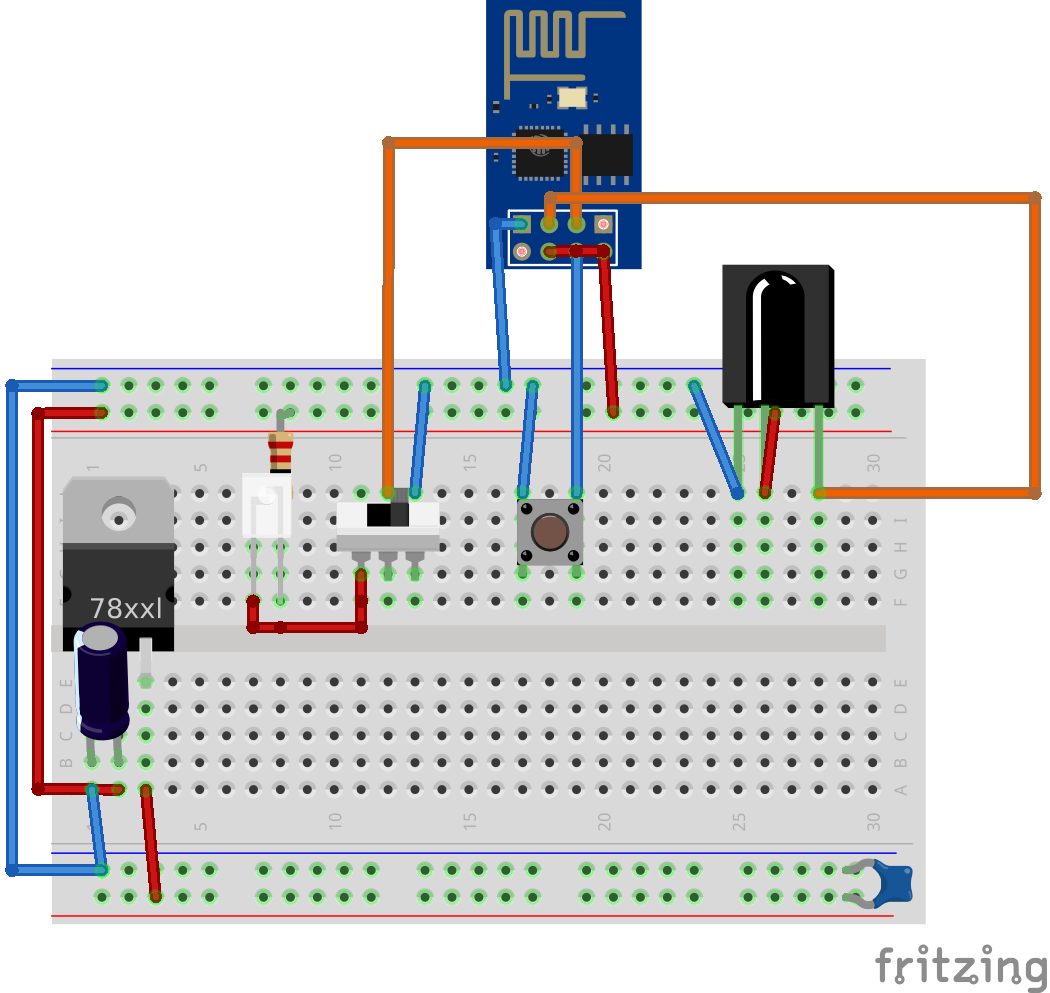
\includegraphics[scale=1]{Abbildungen/ESP8266_Steckplatine}
	\caption{Steckplatine}
\end{figure}

\begin{figure}
	\centering
	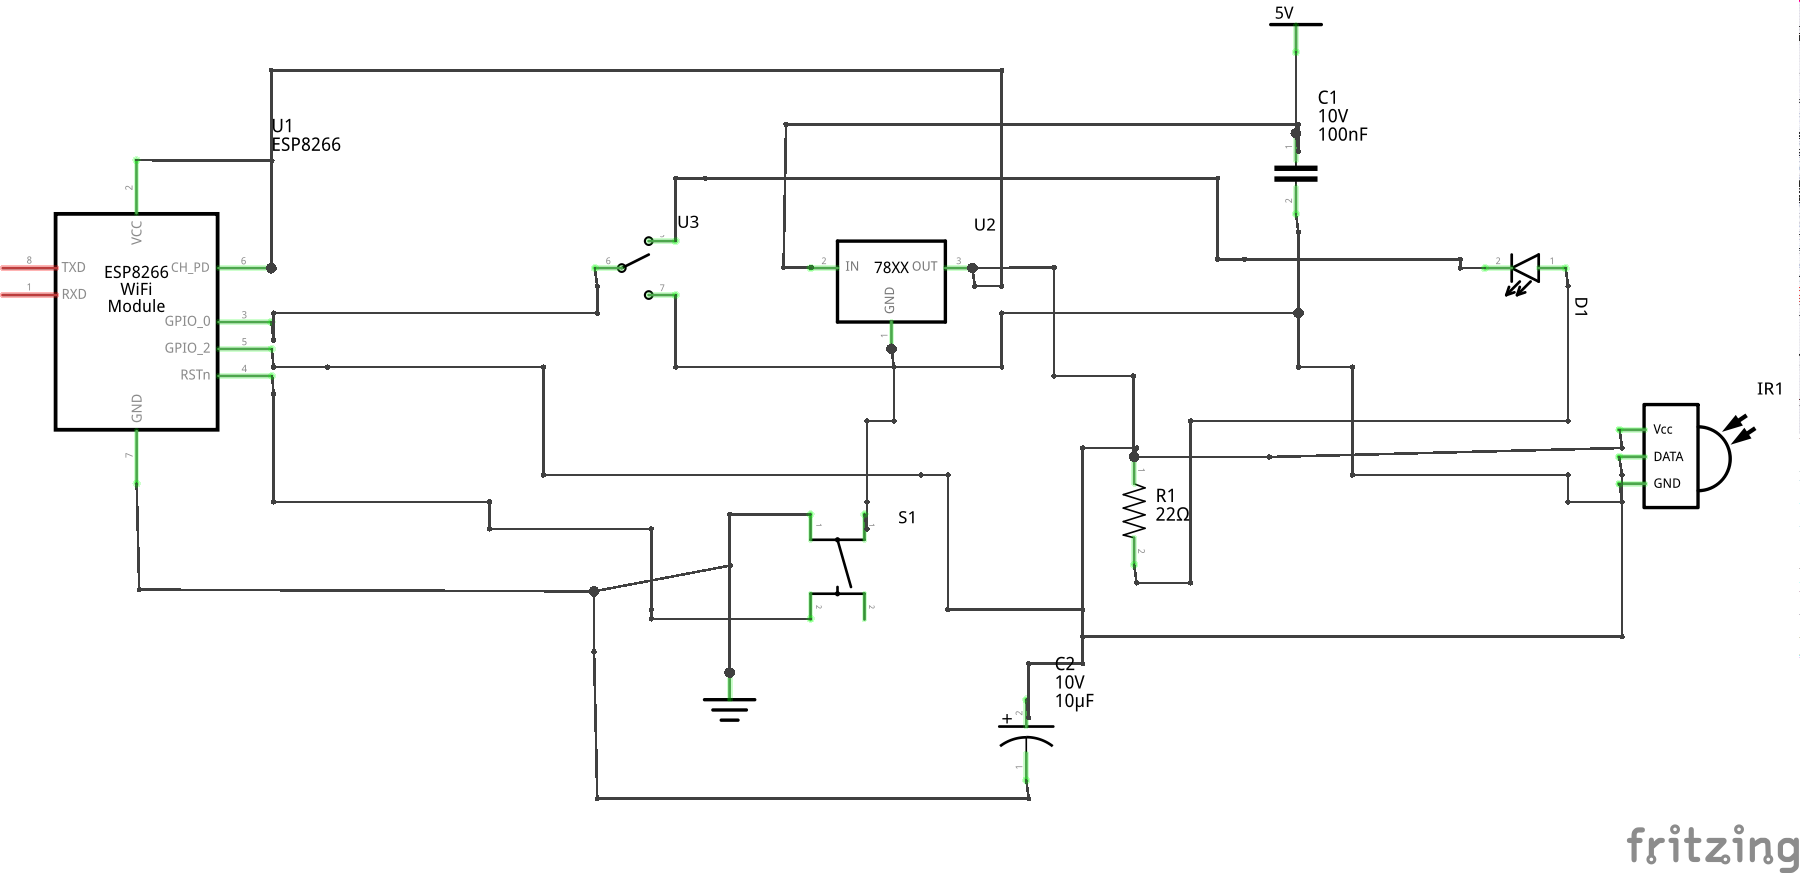
\includegraphics[scale=1]{Abbildungen/ESP8266_Schaltplan}
	\caption{Schaltplan}
\end{figure}


\subsection{Funktionsweise}
\subsubsection{Implementierung}
\section{Zusammenfassung}

\pagestyle{empty}										% Leere Seite 
\end{document}